\section*{\begin{tabular*}{\linewidth}{@{}l @{\extracolsep{\fill}} r@{}}
Nr.~14 & BLK~87/1 \\
\end{tabular*} 
}

\textsf{\textbf{Boleko (Likwala-aux-Herbes; Fpl.~285)}}

\vspace{1em}

\noindent\begin{tabular}{@{}rl@{}}
	\textbf{Feldarbeit:} & \begin{tabular}[t]{@{}l@{}}\textbf{01.08.--04.08.1987}\\ \textbf{(F. Nikulka/H. Holsten)}\end{tabular} \\ 
	\textbf{Abb.:} & \textbf{\ref{fig:BLK87-1_Foto}--\ref{fig:BLK87-1_Metall}} \\ 
	\textbf{Tab.:} & \textbf{\ref{tab:BLK87-1_Funde}}\\
	\textbf{Taf.:} & \textbf{68.4--69.4} \\ 
	\textbf{Lit.:} & \textbf{--} \\ 
\end{tabular} 

\paragraph{Grabung und Befunde}\hspace{-.5em}|\hspace{.5em}%
Im Boleko am unteren \mbox{Likwala}-\mbox{aux}-\mbox{Herbes} (Fpl.~285) wurden bei der Prospektion zwischen zwei Hütten einige an der Oberfläche frei erodierte Gefäße beobachtet. Zudem wurde nach dem groben Putzen der Oberfläche eine längliche Verfärbung sichtbar, in welche die Gefäße eingebettet waren. Der Ost--West-orientierte, knapp 2,5\,m lange und 0,5--0,55\,m breite Befund wurde anschließend unter der Kennung BLK~87/1 ausgegraben (Abb.~\ref{fig:BLK87-1_Skizze}). Ab dem ersten Abtrag ließen sich deutlich drei Bereiche einer Grabgrube unterscheiden (Abb.~\ref{fig:BLK87-1_Skizze}).

Der zentrale Bereich (BLK~87/1-1-2) ist mit dunkelbraunem Lehm und Holzkohle sowie kleinen Partikeln rotegebrannten Lehms verfüllt. Im nördlichen Randbereich befand sich ein dunkler 8--10\,cm breiter, längs des Grubenrandes verlaufender Streifen, der sehr viel Holzkohle enthielt. Der östliche Teil (BLK~87/1-1-3) ist -- im Unterschied zum zentralen Bereich -- mit dunkelgrau-braunem Substrat verfüllt und mit kleinen rotgebrannten Partikeln durchmischt. Ab dem zweiten Abtrag konnten diese beiden Bereiche nicht mehr unterschieden werden.

Im östlichen Bereich (BLK~87/1-1-3) fanden sich zwei fragmentierte Gefäße: unterhalb sowie zwischen einer zerdrückten, rundbauchigen Schale (GE~4; Taf.~68.5) fanden sich die stark zerscherbten Teile einer Flasche mit profilierter Wandung (GE~1; Taf.~69.3).\footnote{Die Flasche war zwar stark zerscherbt, doch war ihre grundsätzliche Orientierung noch erkennbar. Sie lag auf der Seite mit der Mündung nach Norden. Der Befund legt nahe, dass das Gefäß in direktem Zusammenhang mit der Deponierung in der Grabgrube zerschlagen beziehungsweise in die Grube \textit{geworfen} wurde.} Große Fragmente verschiedener Gefäße sind in diesem Bereich und auch in der südlichen Hälfte regelhaft ineinander verschachtelt niedergelegt. Der Bereich war zudem stark mit Holzkohle durchsetzt.

\begin{figure*}[p]
	\centering
	\begin{subfigure}[t]{\textwidth} 
		\centering
		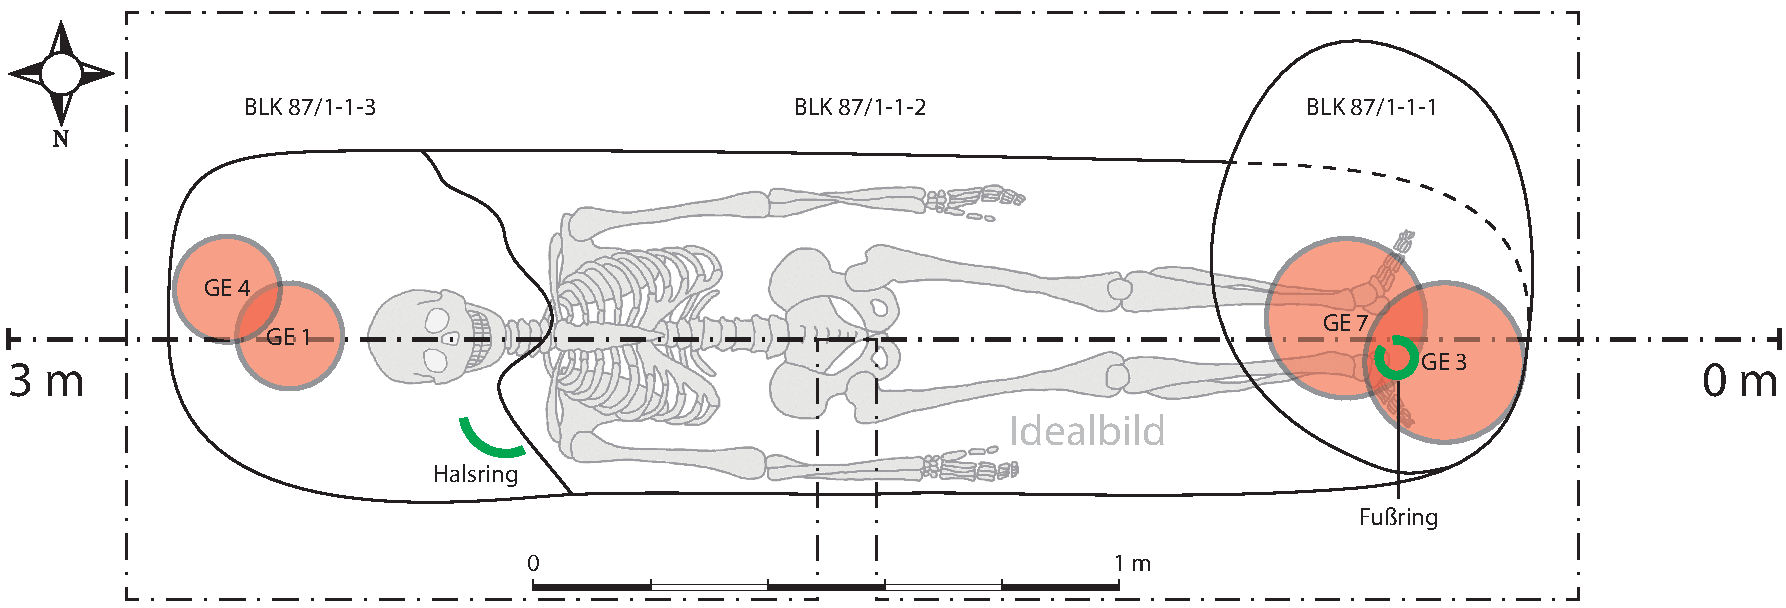
\includegraphics[width = \textwidth]{fig/BLK87-1_Skizzen.pdf}
		\caption{Befundskizze von Süden (Idealbild des Skeletts nach \url{www.digitalefolien.de/biologie/mensch/skelett/skelett1.gif}, Zugriff: 17.06.2013).}
		\label{fig:BLK87-1_Skizze}
	\end{subfigure}
	\begin{subfigure}[t]{\textwidth} 
		\centering
		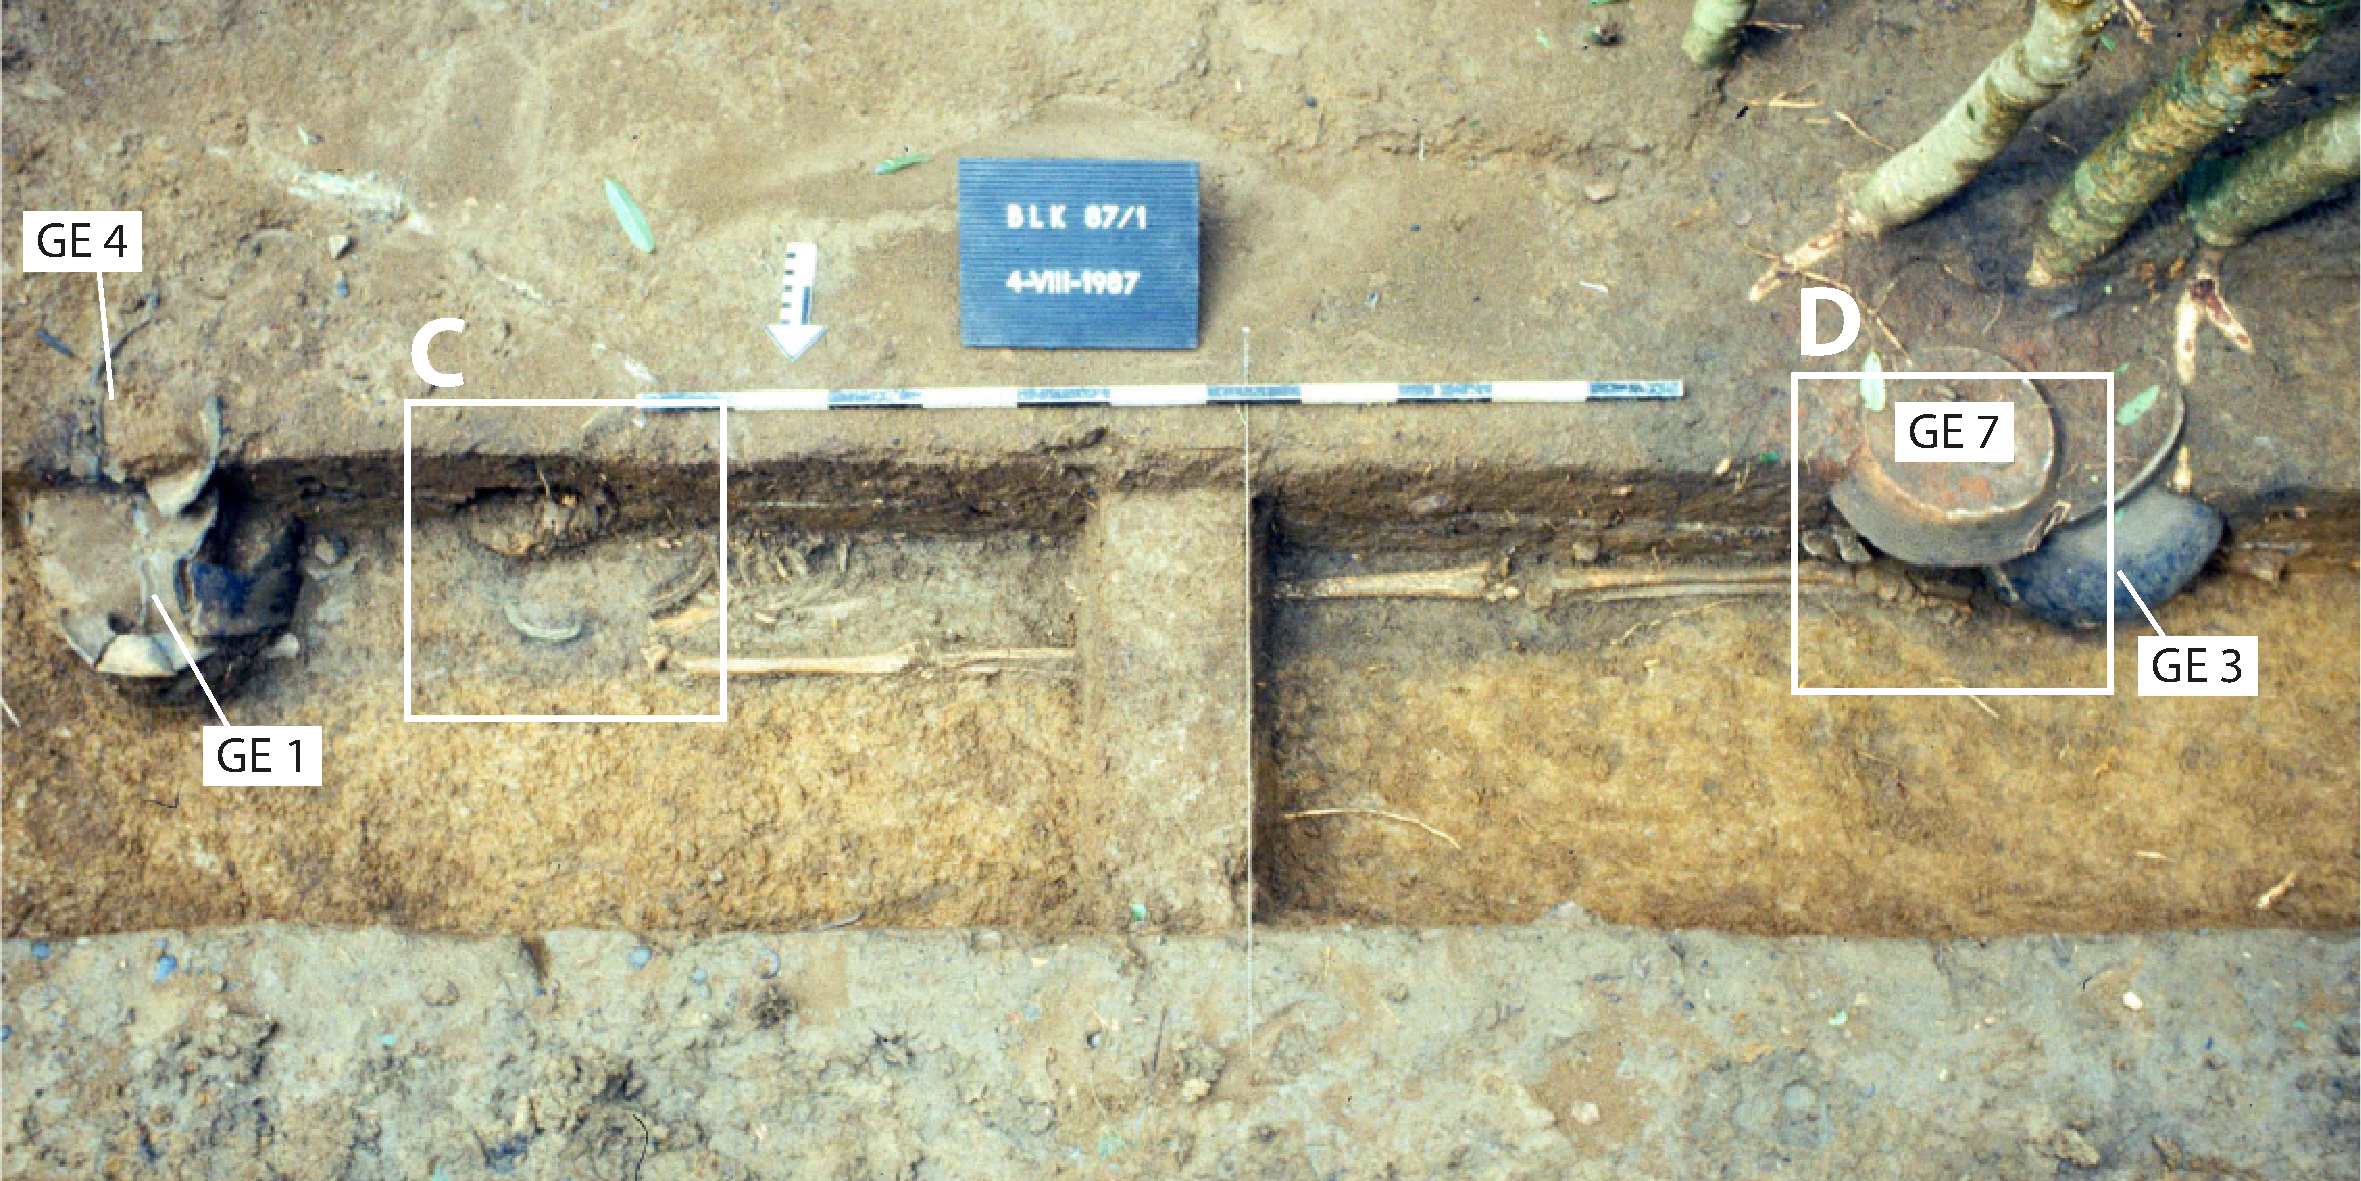
\includegraphics[width = \textwidth]{fig/BLK87-1_F87-01-28.pdf}
		\caption{Abtrag 2 mit dem freigelegten Skelett (von Norden)}
		\label{fig:BLK87-1_Übersicht}
	\end{subfigure}
	\begin{subfigure}[t]{\columnwidth} 
		\centering
		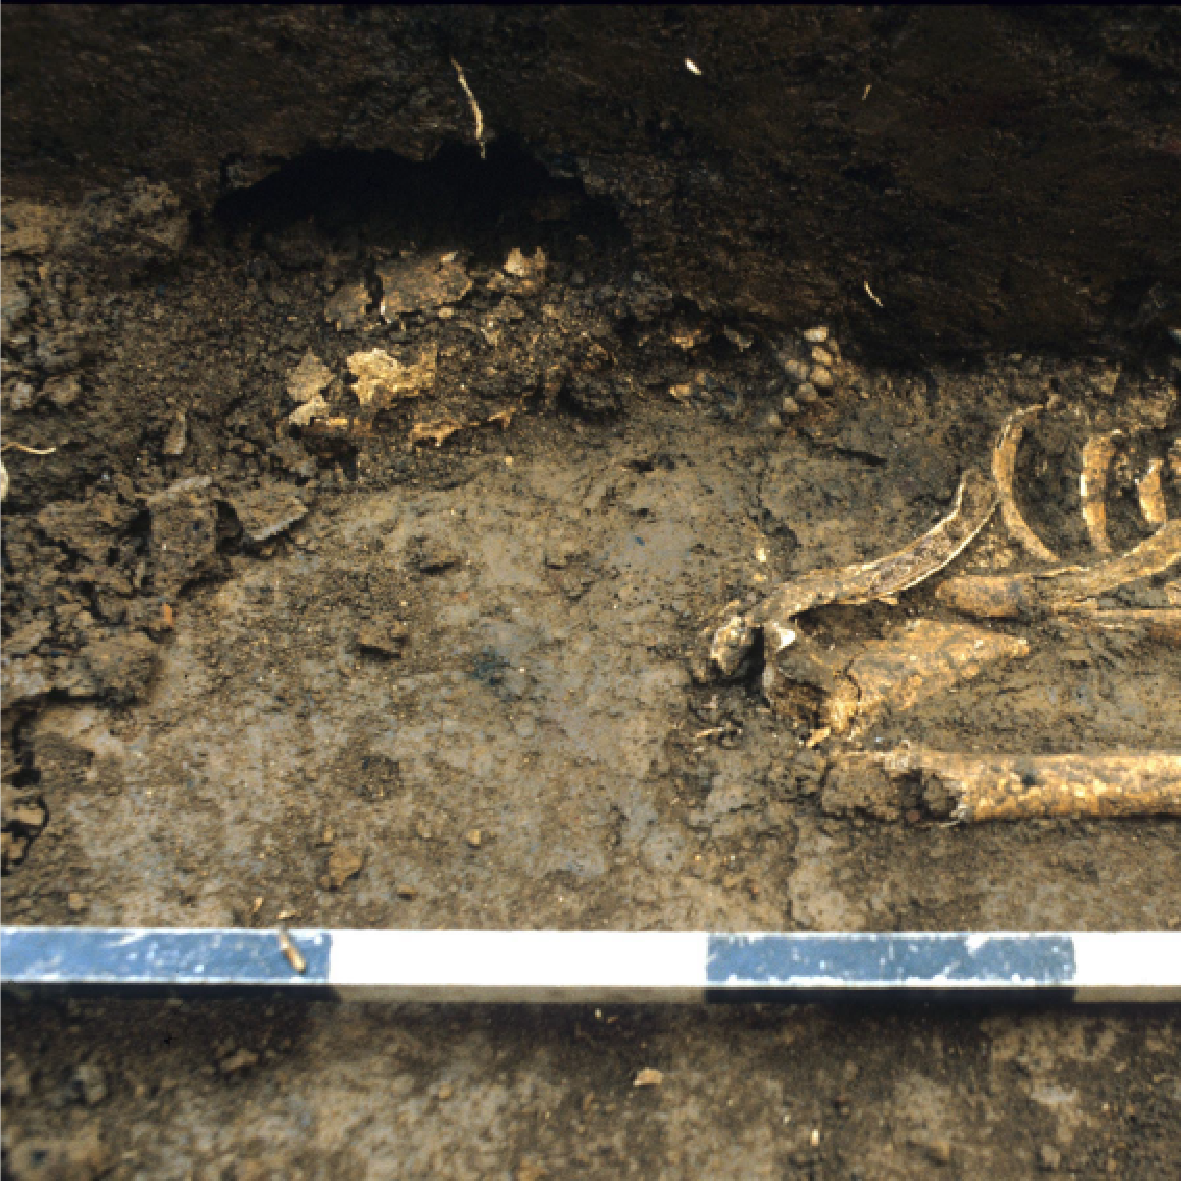
\includegraphics[width = \textwidth]{fig/BLK87-1_F87-01-27.pdf}
		\caption{Detail des Oberkörpers und Schädels. Der Metallring im Bereich der rechten Schulter (siehe a) war zum Zeitpunkt des Fotos bereits entnommen.}
		\label{fig:BLK87-1_Kopfbereich}
	\end{subfigure}\hfill
	\begin{subfigure}[t]{\columnwidth} 
		\centering
		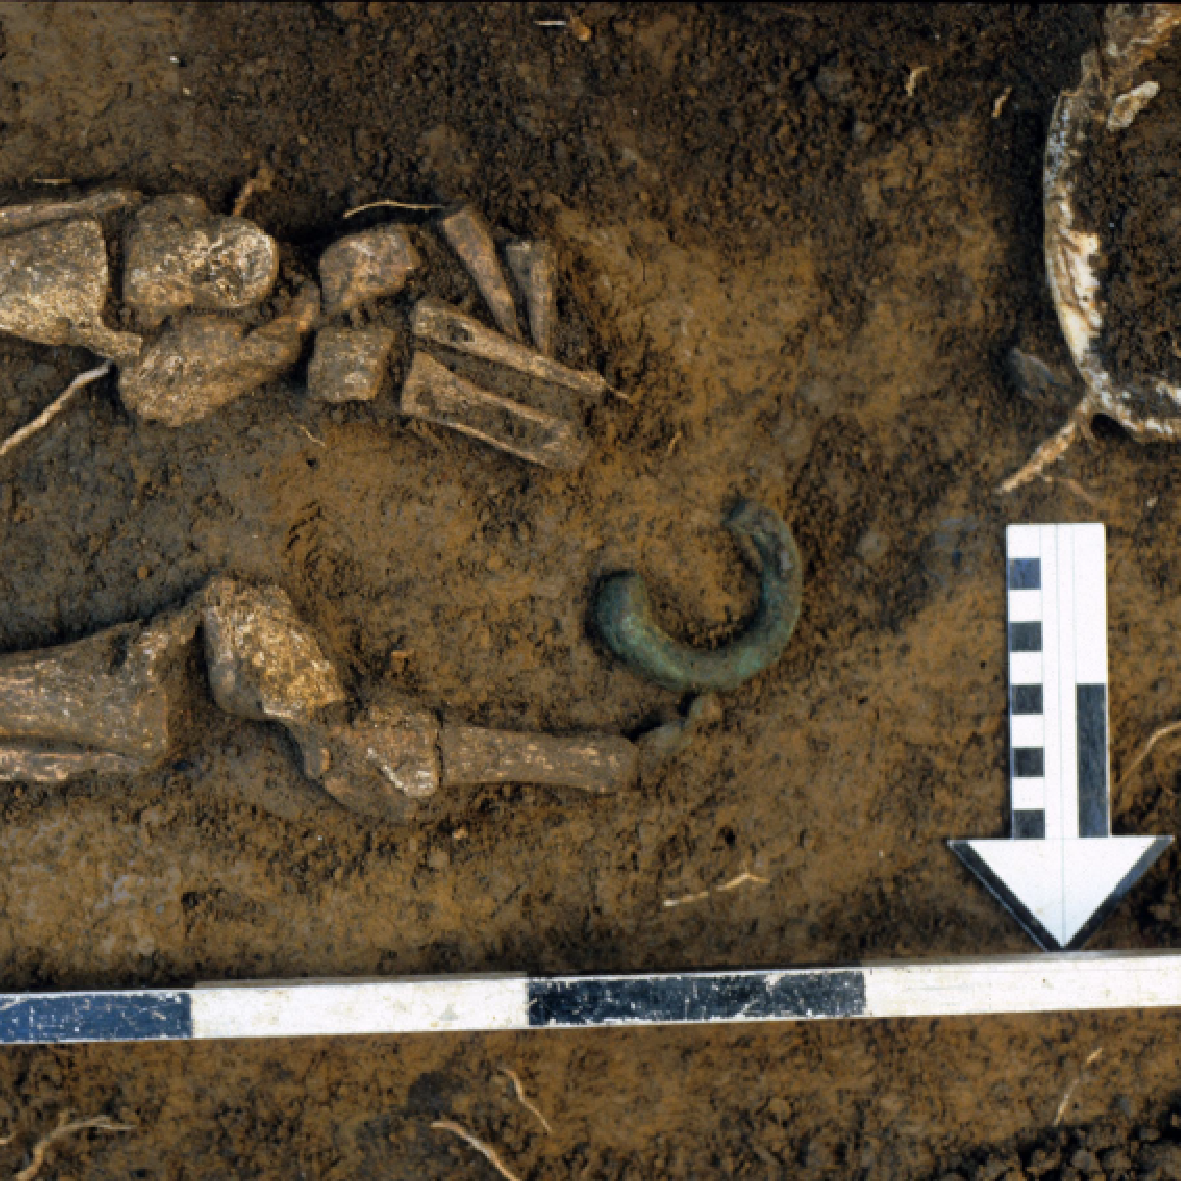
\includegraphics[width = \textwidth]{fig/BLK87-1_F87-02-2.pdf}
		\caption{Details des Fußbereichs mit Messingring unterhalb des Gefäßes GE~3.}
		\label{fig:BLK87-1_Fussbereich}
	\end{subfigure}
	\caption{BLK 87/1: Befund (Fotos: F. Nikulka, 1987).}
	\label{fig:BLK87-1_Foto}
\end{figure*}

Ein westlicher, deutlich abgrenzbare Bereich (BLK~87/1-1-1) wies auffällig viel rotgebrannten Lehm auf, der sich außer- wie innerhalb eines auf seiner Mündung stehenden Gefäßes befand, von dem nur noch der Randbereich erhalten war (GE~7). Unterhalb dieses Gefäßes lag -- komplett erhalten -- ein nahezu aufrecht stehendes, rundbauchiges Gefäß mit ausbiegendem Rand (GE~3; Taf.~68.4). Der westliche Bereich (BLK~87/1-1-1) ist möglicherweise eine jüngere Eingrabung, die in den zentralen Bereich (BLK~87/1-1-2) einschneidet. Die Untergrenze beziehungsweise Sohle der mit rotgebrannten Lehm verfüllten Eingrabung BLK~87/1-1-1 war bereits bei etwa 0,1~m unter der heutigen Oberfläche erreicht. Sicher kann diesem Bereich nur das Randfragment GE~7 zugeordnet werden, während das große Gefäß (GE~3; Taf.~68.4) bis in die Bestattung BLK~87/1-1-2 hineinreicht. Auffällig ist, dass die Gefäße in der westlichen, jüngeren Eingrabung (BLK~87/1-1-1) grundsätzlich intakt deponiert wurden, während die Gefäße im östlichen Bereich bereits zerscherbt in die Grabgrube gelangten oder bei der Deponierung potenziell zerschlagen wurden.

\begin{figure*}[tb!]
	\centering
	\begin{subfigure}{1\textwidth}	
		\centering
		\includegraphics[width=.5\textwidth]{fig/9-11_BLK87-1_VerteilungFunde_R.pdf}
		\caption{Fundkategorien}
		\label{fig:BLK87-1_FundeTypen}
	\end{subfigure}
	\begin{subfigure}{1\textwidth}	
		\centering
		\includegraphics[width=\textwidth]{fig/9-11_BLK87-1_Fragmentierung_2.pdf}
		\caption{Fragmentierung}
		\label{fig:BLK87-1_Keramik_Fragm}
	\end{subfigure}
	\caption{BLK 87/1: Verteilung der Fundmaterialien (A) und Fragmentierungsgrad der Scherben (n~=~7; Größenklassen siehe Anm.~\ref{ftn:Keramik_Fragmentierung}).}
	\label{fig:BLK87-1_Funde}
\end{figure*}

\begin{table*}[tb!]
	\centering
	\begin{minipage}[b]{\columnwidth}
		\centering
		{\footnotesize \begin{sftabular}{@{}lrrrr@{}}
\toprule
\textbf{Fundkategorie} &  \textbf{Anzahl} &    \textbf{\%} &  \textbf{Gewicht (kg)} &    \textbf{\%} \\
\midrule
      Keramik &      58 &  95,1 &          8,07 &  89,9 \\
       Metall &       2 &   3,3 &          0,25 &   2,8 \\
        Stein &       1 &   1,6 &          0,65 &   7,3 \\
\bottomrule
\end{sftabular}
}\vspace{1.5em}
		\caption{BLK~87/1: Anteil verschiedener Fundmaterialien.}
		\label{tab:BLK87-1_Funde}
	\end{minipage}%
	\hfill
	\begin{minipage}[b]{\columnwidth}
		\centering
		{\footnotesize \begin{sftabular}{@{}lrrrrr@{}}
\toprule
\textbf{Befund} & \textbf{BOT} & \textbf{MKA} &   \textbf{EPE} &  \textbf{fraglich} &  \textbf{Summe} \\
\midrule
BLK~87/1-1-1 &        2 & - &   1 & 10 &   13 \\
BLK~87/1-1-2 &        - & - &   - & 8 &    8 \\
BLK~87/1-1-3 &        3 & 1  &  - & 2 &    6 \\
\midrule
Summe      &       5 & 1 &   1 & 20 &   27 \\
\bottomrule
\end{sftabular}
}
		\caption{BLK 87/1: Keramische Stilgruppen.}
		\label{fig:BLK87-1_Keramik_StilGr}
	\end{minipage}
\end{table*}

Ab etwa 0,2\,m unter der Oberfläche traten die ersten Knochen der Bestattung zu Tage: das Individuum lag in Rückenlage mit dem Schädel im Osten (Abb.~\ref{fig:BLK87-1_Skizze}; \ref{fig:BLK87-1_Foto}).\footnote{Der Schädel war zwar bereits zerfallen, jedoch war über ihm noch ein Hohlraum erhalten, was als untrügliches Zeichen für das sehr junge Alter der Bestattung gewertet werden kann. Die Knochen waren sehr gut erhalten und das umgebende Erdreich ließ sich leicht ablösen. Lediglich die \textit{Epiphysen} beziehungsweise Gelenkenden waren stark brüchig.} Die Knochen wurden nicht entnommen. Eine Besonderheit war, dass im Bereich der Füße die Mittelfußknoen (\textit{Metatarsalia}) zwar vorhanden waren, die \textit{Phalangen} jedoch fehlten. Zudem wiesen die \textit{Metatarsalia} an den distalen Gelenkenden leichte Auflösungserscheinungen des Knochens auf (Abb.~\ref{fig:BLK87-1_Fussbereich}).\footnote{Auf Basis der Fotos kann nicht geklärt werden, ob das bestattete Individuum möglicherweise, wie von den Ausgräbern vermutet, an Lepra litt oder die Knochen lediglich durch eine potenziell spätere Deponierung von GE~3 verlagert wurden. Zur Verifizierung dieses Befundes und um mögliche, weitere Beigaben zu finden, wurde der Profilsteg über der rechten Hand abgetragen. Dabei fanden sich nur zwei Fingerknochen, was die Hypothese eines krankheitsbedingten Fehlens der Knochen unterstützt. Im Bereich der Hand wurden keine weiteren Beigaben gefunden.\label{ftn:BLK87-1_Lepra}}

Das Gefäß GE~3 (Taf.~68.4) liegt leicht verkippt direkt zwischen den Füßen beziehungsweise auf dem rechten Fuß. Unterhalb von GE~3, zwischen den beiden Füßen, fand sich ein Messingring (Abb.~\ref{fig:BLK87-1_Metall}.1). Etwa 0,1\,m nördlich des Schädels und 0,1\,m östlich der rechten Schulter wurde ein weiterer Messingring gefunden (Abb.~\ref{fig:BLK87-1_Metall}.2).

\begin{figure*}[tb]
	\centering
	\includegraphics[width=\textwidth]{fig/BLK87-1_Metall.jpg}
	\caption{BLK 87/1: Ringe; zwischen den Füßen (1) und nahe der rechten Schulter (2; Fotos: D. Seidensticker, 2014).}
	\label{fig:BLK87-1_Metall}
\end{figure*}

\paragraph{Keramik\vspace{.5em}}\mbox{}\\
\begin{tabular}{@{}lrl@{}}
Ausgezählt: & 487\,g & \\ 
Bearbeitet: & 8487\,g & (95\,\%) \\ 
Insgesamt: & 8974\,g & \\ 
\end{tabular} 

\vspace{1em}
\noindent Das Keramikinventar aus dem Befund BLK~87/1 setzt sich vor allem aus Gefäßen und großen Gefäßfragmenten zusammen. Diese fanden sich überwiegend in den beiden Keramikkonzentrationen am Ost- sowie Westende des Grabes (Abb.~\ref{fig:BLK87-1_FundeTypen}).

Innerhalb des eigentlichen Grabes (BLK~87/1-1-2) sowie der östlichen Keramikkonzentration (BLK~87/1-1-3) fanden sich, neben einigen wenigen Einzelscherben, vier stark fragmentierte Gefäße: Eine Flasche der Epena-Gruppe (Kap.~\ref{sec:EPE-Gr}) weist den charakteristischen breiten Schulterabsatz und langem Kegelhals auf. Sie weist eine Verzierung aus Rillenbündeln und Eindruckreihen auf (GE~1; Taf.~69.3). Darüber lag eine zerdrückte Schale mit geschweifter Wandung und flächiger \textit{banfwa-nfwa}-Verzierung, deren Randabschluss vom Typ A4.3 starke Bezüge zur Botendo-Keramik des Inneren Kongobeckens aufweist (GE~4; Taf.~68.5; Kap.~\ref{sec:BOT-Gr}). Ebenfalls in diesem Bereich fand sich eine Schale mit gerader, leicht einbiegender Wandung und rundem Boden, die ebenfalls als Vertreter der Botendo-Gruppe angesprochen werden kann (GE~2; Taf.~69.1). Das vierte Gefäß in diesem Bereich ist das Randfragment eines unverzierten, flachen Gefäßes mit ausbiegendem Rand vom Typ E4 (GE~5; Taf.~69.2).

Die potenziell jüngere, westliche Keramikdeponierung (BLK 87/1-1-1) zeichnet sich durch drei wenig verzierte Gefäße aus, von denen zwei nahezu komplett erhalten sind: Ein rundbodiges Gefäß vom Typ E1 weist noch Reste einer aus dunklen, vertikalen Streifen bestehenden Verzierung auf und kann aufgrund dieses Merkmals der Mobaka-Gruppe zugerechnet werden (GE~3; Taf.~68.4; Kap.~\ref{sec:MKA-Gr}). Zwar bereits zur Hälfte erodiert, aber ansonsten intakt war auch der Randbereich einer unverzierten, kleinen Schale (GE~6; Taf.~69.4). Das Fundinventar wurde bereits im Feld der historischen Zeit, dem 19. bis frühen 20.~Jh. n.~Chr. zugeordnet. 

\paragraph{Sonstige Funde}\hspace{-.5em}|\hspace{.5em}%
Neben der Keramik fanden sich im Befund auch zwei metallene Ringe (Abb.~\ref{fig:BLK87-1_Metall}): ein im Querschnitt D-förmiger Ring fand sich zwischen den Füßen des Bestatteten (Abb.\ref{fig:BLK87-1_Foto}; \ref{fig:BLK87-1_Metall}.1), während ein zweiter Ring im Bereich der rechten Schulter lag (Abb.~\ref{fig:BLK87-1_Metall}.2).\footnote{Der zwischen den Füßen der Bestattung gefundene Ring (Abb.~\ref{fig:BLK87-1_Metall}.1) weist einen Durchmesser von 4,5\,cm (innen) bis 7\,cm (außen) auf. Dieser Ring ist 14\,mm breit und 13\,mm dick. Der zweite, nahe der rechten Schulter gefundene Ring (Abb.~\ref{fig:BLK87-1_Metall}.2) weist einen Durchmesser von etwa 11\,cm auf, ist 13\,mm breit und 11\,mm dick. Im Querschnitt ist auch er D-förmig, mit einer inneren, gerundeten und einer äußeren geraden Seite. Innen lassen sich weiße bis rötlich-violette Anhaftungen beobachten.} Es muss offen bleiben, ob der zweite Ring ursprünglich einmal geschlossen war.\footnote{Zur Funktion von Eisenobjekten in Gräbern siehe \textcites{GonzalezRuibal.2011}[124--126]{Eggert.2016} sowie \textcite[siehe][]{Ballarini.2009} für einen umfassenden Katalog von vergleichbaren Metallobjekten in Afrika.}

\paragraph{Anthropologie}\hspace{-.5em}|\hspace{.5em}%
Die Knochen wurden nicht geborgen und stehen daher nicht für anthropologische Untersuchungen zur Verfügung. Der schriftlichen und fotografischen Dokumentation ist zu entnehmen, dass das Individuum zwischen 1,7--1,8\,m groß war. Als Auffälligkeiten müssen die fehlenden Finger- und Fuß-Phalangen genannt werden. Ob dies ein Zeichen krankheitsbedingter Veränderungen ist, kann auf Basis der Fotos nicht entschieden werden.\footnote{Siehe Anm.~\ref{ftn:BLK87-1_Lepra}.}

\paragraph{Datierung}\hspace{-.5em}|\hspace{.5em}%
Eine direkte Datierungen für das Grab liegt nicht vor. Die mit dem Befund assoziierte Keramik ist sämtlich als rezent bis sub-rezent ansprechbar und der Umstand, dass über dem zusammengefallenen Schädel noch ein Hohlraum erhalten war, deutet ein deutlich junges Alter der Bestattung an. Der Befund wird als Konsequenz dieser Beobachtungen als rezent bis sub-rezent angesprochen und datiert wohl in einen Zeitraum zwischen dem Ende des 19. und der Mitte des 20.~Jh. n.~Chr.

\begin{figure*}[!tb]
	\begin{minipage}[b]{.66\textwidth}
		\includegraphics[width=\textwidth]{fig/MUN87_Fpl-Plan.pdf}
	\end{minipage}\hfill
	\begin{minipage}[b]{.3\textwidth}
		\caption{Munda (Fpl.~304): Übersichtsplan.}\label{fig:MUN87_Fundstelle}
	\end{minipage}
\end{figure*}

\paragraph{Interpretation}\hspace{-.5em}|\hspace{.5em}%
Die Grabung BLK~87/1 erfasste das rezente bis sub-rezente Grab eines zwischen 1,7--1,8\,m großen Individuums. Das Grab ist nahezu exakt Ost--West ausgerichtet, wobei der Kopf im Osten liegt. Am Kopf wie am Fußende finden sich zwei Konzentrationen von Keramik, wobei die am Fußende befindlichen Gefäße potenziell in einer separaten Eingrabung deponiert wurden. Die gefunden Gefäße sind den Stilgruppen Epena (Kap.~\ref{sec:EPE-Gr}), Mobaka (Kap.~\ref{sec:MKA-Gr}) sowie Botendo (Kap.~\ref{sec:BOT-Gr}) zuzuordnen. Neben der Schulter sowie dem Fußende der Bestattung fand sich jeweils ein metallener Ring.